\chapter{Marco teórico y Estado del arte}
\label{ch:estado del arte}

\quad El problema del procesamiento de imágenes para su restauración y escalado lleva tratándose desde hace décadas. A lo largo de este tiempo, se han desarrollado diferentes técnicas y algoritmos. Se llamará modelo clásico a todos los algoritmos y técnicas que se desarrollaron antes de la popularización de las las redes de neuronas.

\section{Modelo Clásico: Restauración}

\quad El deterioro en las imágenes es un factor que puede afectar su captura. Este deterioro puede manifestarse de distintas formas, como desenfoque de movimiento, presencia de ruido o fallos en el dispositivo de captura\cite{OWLNet}.

El deterioro se puede representar matemáticamente de la siguiente forma\cite{Wavelet}:

\begin{equation}
	y = D*X + n \label{eq:detfunc}
\end{equation}

Donde $X$ es la imagen original, $D$ es la función de desenfoque (o filtro paso bajo) y $n$ es el ruido que se le añade a la imagen. En \eqref{eq:detfunc}, $y$ es la imagen resultante de aplicar las transformaciones.
Un ejemplo simple de función en el modelo clásico es el \textbf{filtro inverso}. Este método parte de: 
	
\begin{equation}
	g = X*b \label{eq:convfilterfunc}
\end{equation}
Donde $g$ es la imagen borrosa y $b$ es un filtro paso bajo.

Esta aproximación aplica una convolución $*$ de la imagen borrosa $g$ con un filtro de paso alto $h$ para recuperar la imagen original:
	
\begin{equation}
	X = g*h \label{eq:invfilterfunc}
\end{equation}

\begin{figure}[H]
	\centering
	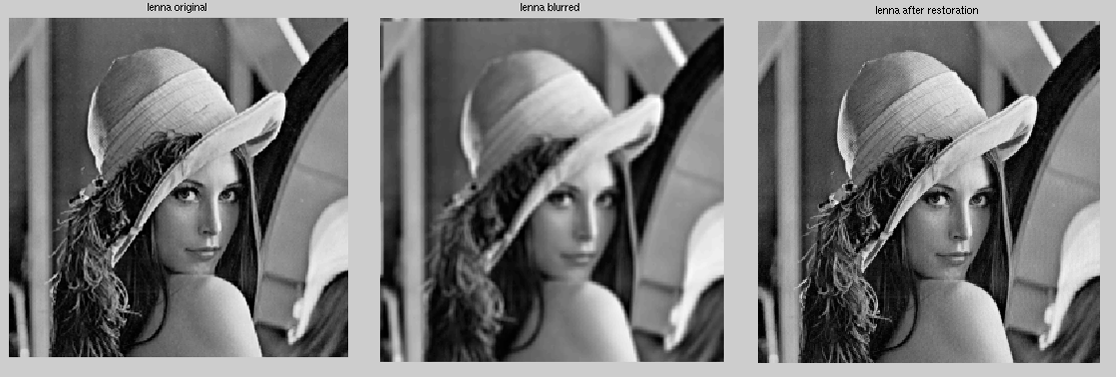
\includegraphics[width=0.6\textwidth]{figures/lenna_inverse_dir_blur.png}
	\caption{\label{fig:lenna_inverse_dir_blur}Imagen comparativa del uso del filtro inverso en una imagen con desenfoque. Fuente: \cite{OWLNet_inverse}}
\end{figure}
	
	Sin embargo, el filtrado inverso responde negativamente ante la presencia de ruido:
	
\begin{figure}[H]
	\centering
	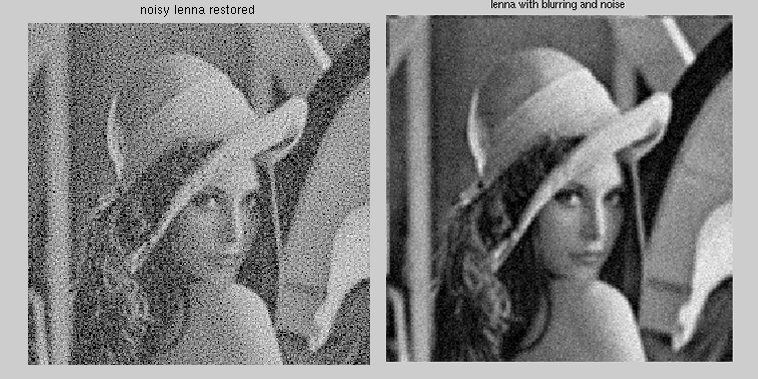
\includegraphics[width=0.5\textwidth]{figures/lenna_inverse_dir_noise.png}
	\caption{\label{fig:lenna_inverse_dir_noise} Imagen comparativa del uso del filtro inverso en una imagen con ruido. Fuente: \cite{OWLNet_inverse}}
\end{figure}


Este algoritmo necesita saber cuál es la función de paso bajo. Existen otras aproximaciones llamadas \textbf{deconvoluciones a ciegas} que no necesitan esta información, con tan solo la imagen pueden funcionar. Un ejemplo es el método \gls{pse} que busca restaurar la distribución original de la energía en el espectro de frecuencias, lo que puede mejorar la claridad y calidad de la imagen. Esto se logra aplicando filtros o técnicas de procesamiento que ajustan la amplitud de las diferentes frecuencias para igualarlas a un espectro de referencia deseado\cite{OWLNet_blind}.

Su fórmula principal es:

\begin{equation}
G = [\frac{S_{uu}}{|H|^2S_{uu}+S_{nn}}]^{1/2}\label{eq:PSE}
\end{equation}
	
Donde $H$ es la transformada de Fourier de $h$ (la función de paso bajo). Este es el parámetro que se quiere estimar para hallar una imagen $G$ sin deterioro. $S_{uu}$ es la densidad espectral y $S_{nn}$ es el ruido espectral. Ambos son parámetros que se supone que se conocen o se pueden estimar, aunque los resultados no son los mejores:

\begin{figure}[H]
	\centering
	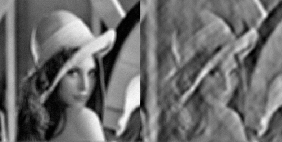
\includegraphics[width=0.5\textwidth]{figures/lenna_blind_deconv.png}
	\caption{\label{fig:lenna_blind_deconv}Imagen comparativa del uso de la deconvolución a ciegas. Fuente: \cite{OWLNet_blind}}
\end{figure}

\section{Modelo Clásico: Escalado}

\quad En el problema del escalado de imágenes, existen varias técnicas de interpolación. La interpolación es una técnica que consiste en rellenar y añadir nuevos píxeles a una imagen únicamente con la información de la misma \cite{matlabinterpolation}.

Si se tiene una imagen como esta:

\begin{figure}[H]
	\centering
	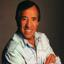
\includegraphics[width=0.3\textwidth]{figures/fary.jpg}
	\caption{\label{fig:fary}Imagen de El Fary reescalada a 64x64. Fuente: \cite{fary}}
\end{figure}

Una primera aproximación sería separar los puntos y rellenarlos con los píxeles que hay alrededor, a este proceso se le conoce como \textit{\textbf{Nearest Neighbor}}:

\begin{figure}[H]
	\centering
	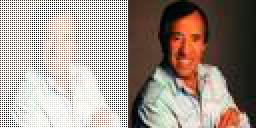
\includegraphics[width=0.6\textwidth]{figures/fary_ampliada.png}
	\caption{\label{fig:farynearneighbour}Proceso de \textit{Nearest Neighbor}. Fuente: Elaboración propia.}
\end{figure}

El resultado no es más que una imagen con píxeles más grandes y no consigue verse con mejor resolución. Se puede mejorar rellenando los huecos con la media entre los puntos, esta aproximación la utilizan la interpolación bilinear y la bicúbica:

\begin{figure}[H]
	\centering
	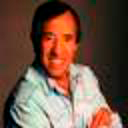
\includegraphics[width=0.3\textwidth]{figures/fary_ampliada_bilinear.png}
	\caption{\label{fig:farybilinear}Escalado con bilinear. Fuente: Elaboración propia.}
\end{figure}

\section{Modelo Actual}

\quad Como se ha visto en la sección anterior, los algoritmos clásicos para restaurar imágenes son ineficientes y requieren información adicional que debe ser estimada mediante cálculos muy complejos. En cuanto a los modelos para escalar imágenes, no logran obtener una resolución satisfactoria.

El principal inconveniente de estas aproximaciones de restauración y escalado es que no pueden generar datos que no existen en la imagen original. Es decir, no pueden proporcionar información que la imagen en sí misma no contenga. Para abordar este desafío, se recurre a las redes neuronales.

Aunque las redes de neuronas fueron propuestas en 1943 por McCulloch y Pitts\cite{neuronaartificial}, no ha sido hasta ahora, gracias a los avances en la tecnología y en el campo de la inteligencia artificial, que es posible crear modelos complejos de redes capaces de reconocer patrones complicados en los datos de entrada. 

Las redes de neuronas artificiales intentan imitar el comportamiento de las neuronas biológicas. Es decir, las neuronas reciben estímulos (cálculos matemáticos) y generan una salida. Estas constan de cinco partes: las entradas $x_i$, la salida $y$, los pesos $w_i$, el \textit{bias} $b$ y la función de activación $a$\cite{neuronaartificial,neuronaibm}.

\begin{figure}[H]
	\centering
	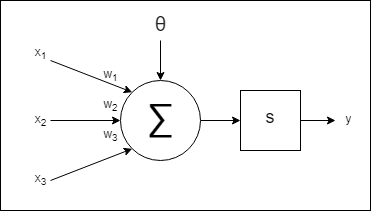
\includegraphics[width=0.4\textwidth]{figures/neurona_artificial.png}
	\caption{\label{fig:neuronaartificial}Neurona Artificial. Fuente: Elaboración propia.}
\end{figure}

Si se juntan más neuronas, forman lo que se llama \textbf{perceptrón multicapa}. Este modelo tiene la siguiente estructura: una capa de entrada, una o muchas capas ocultas y una capa de salida\cite{neuronaibm}.

\begin{figure}[H]
	\centering
	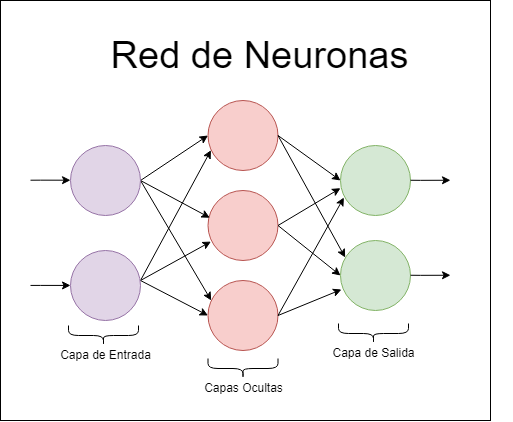
\includegraphics[width=0.5\textwidth]{figures/neural_network.png}
	\caption{\label{fig:neuralnetwork}Red de neuronas. Fuente: Elaboración propia.}
\end{figure}

Existen tres fases principales en las redes de neuronas: la inferencia o propagación, el cálculo del error y la retropropagación. 

La \textbf{inferencia} sirve para generar un resultado a partir de unas entradas. El algoritmo es el siguiente: se multiplica cada entrada $x_i$ por su peso $w_i$ y luego se suma cada producto pasando el resultado a la función de activación $a$ que genera una salida $y$. 

El \textbf{cálculo del error} consisten en comparar la salida de la red con el valor objetivo al que se quiere llegar. Existen distintos tipos de errores, los mas comunes son: \gls{mae} y \gls{mse}.

En la \textbf{retropropagación}, se ajustan los pesos $w_i$ para que la red pueda adaptarse a su tarea\cite{goodfellow}. La fórmula es la siguiente:

\begin{equation}
	\varDelta w_i = w_i-\alpha·\delta_i\label{eq:backpropagation}
\end{equation}

Donde $\alpha$ es el factor de aprendizaje o \textit{learning rate} Indica cómo de rápido tiene que ajustarse el modelo.

\subsection{Redes Convolucionales}

\quad Entendiendo cómo funcionan las redes de neuronas, si se translada al problema de este \gls{pfg}, es decir, trabajar con imágenes, siguiendo el modelo anterior, se tendría que aplanar la imagen para pasarla a la red de neuronas, cosa que supondría dos principales problemas:

\begin{enumerate}
	\item Para imágenes grandes, el número de neuronas necesario para cada píxel escala de forma exponencial. Es decir, si se tiene una imagen de 1024x1024, las neuronas de entrada serían 1.048.576.
	\item Esta distribución hace que se pierda la información espacial de la imagen. El primer pixel de la imagen está relacionado con el último, cuando estos no tienen ninguna relación.
\end{enumerate}

\begin{figure}[H]
	\centering
	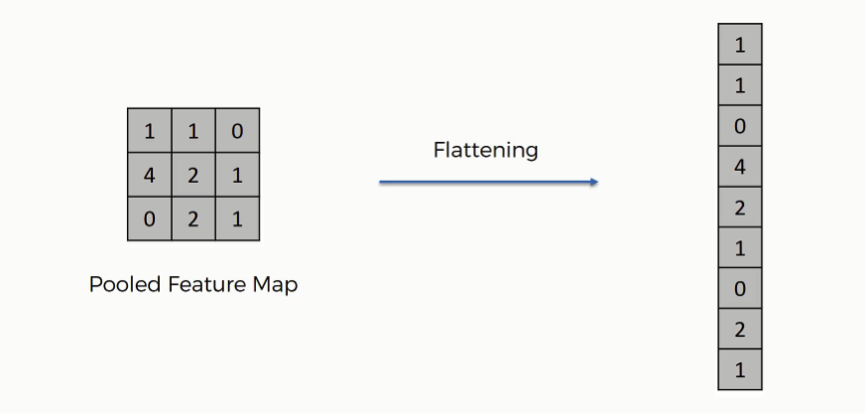
\includegraphics[width=0.4\textwidth]{figures/flatten.png}
	\caption{\label{fig:flatten}Aplanar una imagen para la entrada de una red de neuronas. Fuente: \cite{flatten}}
\end{figure}

Teniendo todo esto en cuenta, se hace necesaria la creación de otro tipo de redes orientadas a imágenes con el fin de reducir la dimensionalidad de la red y evitar la pérdida de información espacial de la imagen. Las redes convolucionales surgen para abordar este tipo de problema.

Las \textbf{\gls{cnn}} tienen sus raíces en el modelo \textit{Neocognitron}, desarrollado por Kunihiko Fukushima en 1980, que sentó las bases para el reconocimiento de patrones a través de estructuras jerárquicas\cite{neocognitron}. Posteriormente, en 1998, Yann LeCun y sus colaboradores introdujeron el uso de la retropropagación para el entrenamiento eficaz de estas redes\cite{LeCun1998}.

\begin{figure}[H]
	\centering
	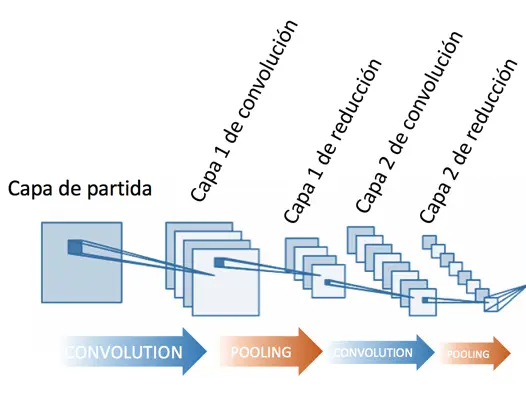
\includegraphics[width=0.5\textwidth]{figures/red-neuronal-convolucional-arquitectura.jpg}
	\caption{\label{fig:cnnarq}Arquitectura de una \acrfull{cnn}. Fuente: \cite{Calvo}}
\end{figure}

Las \textbf{\acrlong{cnn}} extraen características de las imágenes mediante capas compuestas por diferentes filtros del mismo tamaño, cada uno de los cuales contiene pesos $w_i$. Estas redes neuronales aprenden qué filtros son los más efectivos para extraer las características relevantes de las imágenes.

\begin{figure}[H]
	\centering
	\includegraphics[width=0.4\textwidth]{figures/convolución.jpg}
	\caption{\label{fig:convolucion}Operación de convolución. Fuente: \cite{Calvo}}
\end{figure}

Para reducir la dimensionalidad de la imagen manteniendo la información importante, se puede utilizar una técnica llamada \textit{pooling}. El \textit{pooling} aplica un operador a pequeñas subregiones de la imagen, llamadas \textit{kernels}, para combinar sus valores y producir una única salida\cite{Calvo}. Existen dos variantes principales de \textit{pooling}:
\begin{itemize}
	\item \textbf{\textit{MaxPooling}}: Selecciona el valor más grande dentro de cada subregión del \textit{kernel}, reteniendo la característica más prominente de esa región.
	\item \textbf{\textit{AveragePooling}}: Calcula el valor promedio de los elementos en cada subregión del \textit{kernel}, obteniendo una representación suavizada.
\end{itemize}

El uso del \textit{pooling} ayuda a reducir el tamaño de las representaciones intermedias en la red, disminuyendo la cantidad de parámetros y la carga computacional.

\begin{figure}[H]
	\centering
	\includegraphics[width=0.4\textwidth]{figures/reducción.jpg}
	\caption{\label{fig:maxpooling}Operación de MaxPooling. Fuente: \cite{Calvo}}
\end{figure}

También existe la operación contraria llamada \textit{transpose convolution}:

\begin{figure}[H]
	\centering
	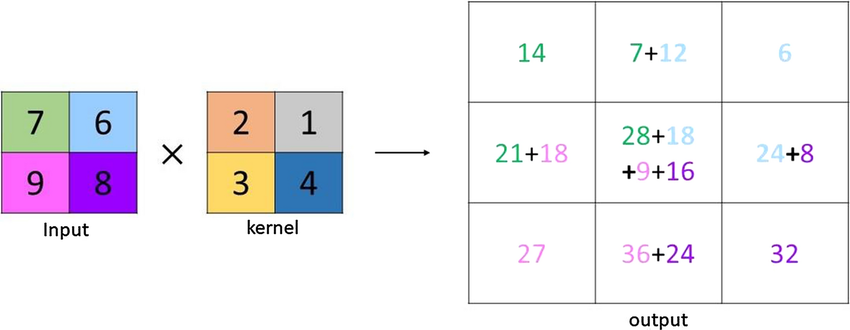
\includegraphics[width=0.7\textwidth]{figures/Transpose-Convolution.png}
	\caption{\label{fig:transposecv}Transpose Convolution. Fuente: \cite{transposecv}}
\end{figure}

Esta operación es útil para \textbf{escalar} una imagen.

\subsection{Arquitecturas de redes de neuronas}

\quad Una arquitectura de red de neuronas se refiere a la estructura organizativa de las neuronas artificiales y las conexiones entre ellas\cite{arqnn}. Existen distintos tipos de arquitecturas como:

\subsubsection{Autoencoders}
\quad Los \textbf{autoencoders} fueron propuestos por primera vez por Kramer en 1991 como una forma de redimensionar datos\cite{autoencoder,michelucci2022autoencoders}. Los autoencoders constan de tres partes: el codificador, el espacio latente y el decodificador.

\begin{figure}[H]
	\centering
	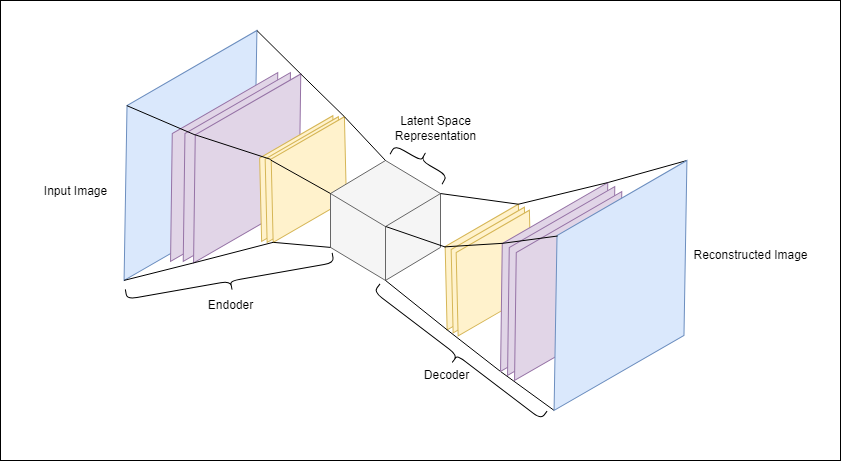
\includegraphics[width=0.7\textwidth]{figures/latent_representation_AE.png}
	\caption{\label{fig:latentrepresentation}Autoencoder. Fuente: Elaboración Propia.}
\end{figure}

El \textbf{codificador} o en ingles \textit{encoder} se puede representar de la siguiente forma\cite{michelucci2022autoencoders}:

\begin{equation}
	h_i = g(X_i) \quad \text{donde } h_i \in R^q \text{ simboliza el espacio latente.} \label{eq:autoencoder1}
\end{equation}

El \textbf{decodificador} o en ingles \textit{decoder} se puede representar de la siguiente forma:

\begin{equation}
	\tilde{x}_i = f(h_i) = f(g(x_i)) \quad \text{donde } \tilde{x}_i \in R^n \label{eq:autoencoder2}
\end{equation}

Para el entrenamiento del autoencoder, hay que buscar las funciones f y g que minimicen la diferencia entre $x_i$ y $\tilde{x}_i$:
\begin{equation}
	argmin_{f,g} <[∆(x_i,f(g(x_i)))]> \label{eq:autoencoder3}
\end{equation}

\subsubsection{VAEs}
\quad Los \textbf{\glspl{vae}} fueron introducidos por primera vez en 2013 por Diederik P. Kingma y Max Welling\cite{vae}. Los \glspl{vae} usan la capacidad de los autoencoders para aprender representaciones eficientes de datos con principios de inferencia variacional, permitiendo la generación de nuevos datos similares a los de entrenamiento.

En los \glspl{vae}, se trabaja con dos tipos de variables: las observables y las latentes. Las variables latentes son variables que están dentro del modelo y capturan las características subyacentes de los datos.

Sea $x\in X^D$ un vector de variables observables, donde $X \subseteq R$ y sea $z\in R^M$ un vector de variables latentes. Para ver cómo las variables latentes generan las variables observables, se necesita la probabilidad conjunta de $x$ y $z$.

\begin{equation}
	p_\theta(x,z)dz \label{eq:vae1}
\end{equation}

Para sacar la distribución marginal con las propiedades de la probabilidad conjunta para datos continuos se tiene\cite{vae,vae2}: 

\begin{equation}
	p_\theta(x)=\int {p_\theta(x,z)dz} \label{eq:vae2}
\end{equation}

Para entrenar el modelo es necesario despejar z cosa que computacionalmente es imposible de tratar, así que, se opta por otra solución: intentar maximizar la función \gls{elbo}\cite{vae,vae2}:

\begin{equation}
\text{ELBO} => \ln{p_\theta(x)} \le E_{z\text{\textasciitilde}q_\phi(z/x)}[\ln{p_\theta(x/z)} + \ln{p_\theta(z)} - \ln{q_\phi(z/x)}] \label{eq:elbo}
\end{equation}

\begin{itemize}
	\item Donde $q_\phi(z/x)$ es el \textbf{codificador}.
	\item Donde $p_\theta(x/z)$ es el \textbf{decodificador}.
	\item Donde $p_\lambda(z)$ es el prior o la \textbf{similitud marginal}.
\end{itemize}

\begin{figure}[H]
	\centering
	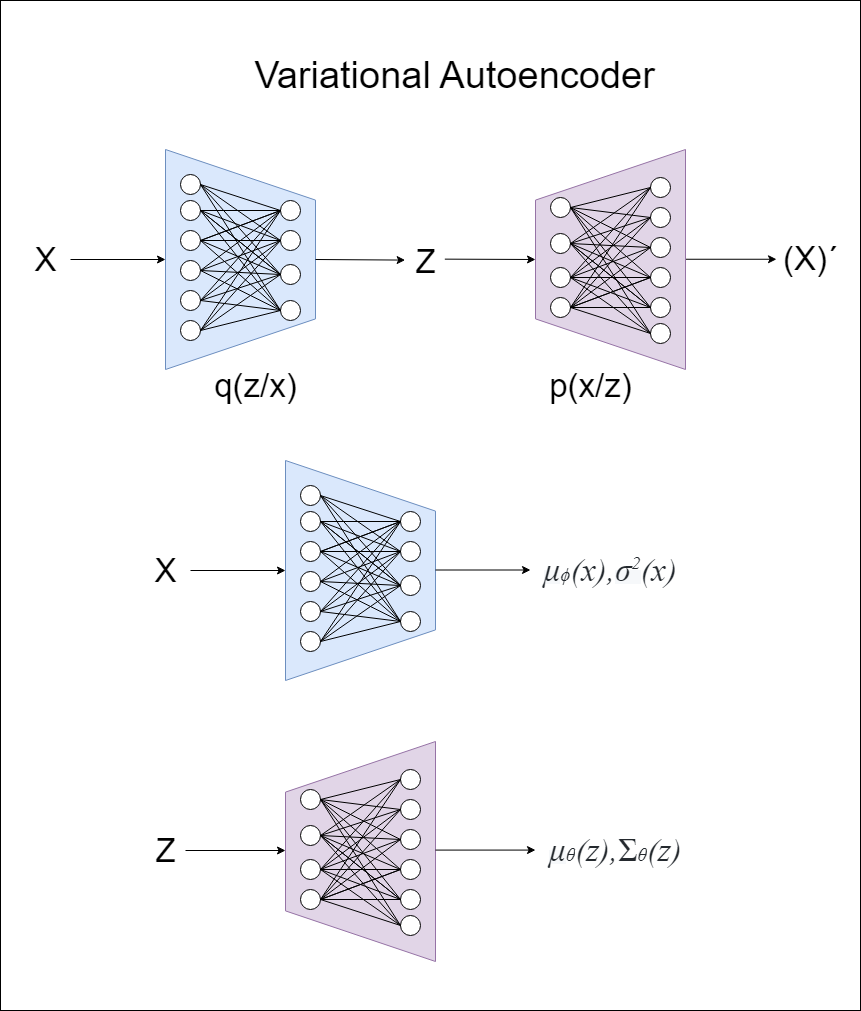
\includegraphics[width=0.7\textwidth]{figures/variational_autoencoder_model.png}
	\caption{\label{fig:vaerepresentation} Representación de un variational autoencoder. Fuente: Elaboración Propia.}
\end{figure}

\subsubsection{GANs}
\quad Las \textbf{redes generativas adversarias} o \textbf{\glspl{gan}}, presentada por Ian Goodfellow en 2014\cite{gan}, han representado un avance significativo en el campo de la Inteligencia Artificial generativa. Esta arquitectura consta de dos redes neuronales que compiten por producir resultados óptimos. La primera red es la \textbf{generadora}, que busca crear imágenes realistas, mientras que la segunda es la \textbf{discriminadora}, encargada de distinguir entre imágenes reales y generadas.

\begin{figure}[H]
	\centering
	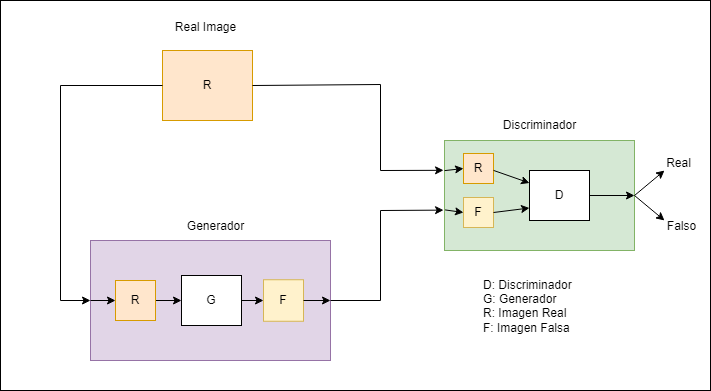
\includegraphics[width=0.8\textwidth]{figures/Basic_GAN.png}
	\caption{\label{fig:basicgan} Representación de una red \gls{cgan}. Fuente: Elaboración Propia.}
\end{figure}

La fórmula general de las redes GAN parte de la fórmula de la entropía cruzada binaria o binary cross entropy:

\begin{equation}
	L = -\sum y\ln(\hat{y}) + (1-y)\ln(1-\hat{y}) \label{eq:gan1}
\end{equation}

\begin{itemize}
	\item Si  $y = 1$; \quad $\hat{y} = D(x) \Rightarrow L = \ln[D(x)]$
	\item Si  $y = 0$; \quad $\hat{y} = D(G(z)) \Rightarrow L = \ln[1 - D(G(z))]$
\end{itemize}

Entonces substituyendo sobre \ref{eq:gan1} nos queda: 
\begin{equation}
	L = \ln[D(x)] + \ln[1 - D(G(z))] \label{eq:gan2}
\end{equation}

Si aplicamos la esperanza en toda la igualdad:
\begin{equation}
	E(L) = E(ln[D(x)]) + E(ln[1-D(G(z))]) \label{eq:gan3}
\end{equation}

Aplicando las propiedades de la esperanza para valores continuos:
\begin{equation}
 	E[X] = \int_{R} Xf(X)dx =>  \int P_{datos}(x) (ln[D(x)])dx + \int P_{z}(z)(ln[1-D(G(z))])dz \label{eq:gan4}
\end{equation}

Reescribiendo la ecuación \ref{eq:gan4} queda esta expresión en la que ambas funciones compiten, ya que, la función G quiere minimizarla y D maximizarla:
\begin{equation}
 min_G max_D V(G,D) = E_{x\text{\textasciitilde}P_{datos}}[ln(D(x))] + E_{z\text{\textasciitilde}Pz}[ln(1-D(G(z)))] \label{eq:gan5}
\end{equation}
